\section*{Michał Śnieg}

\section{Wyrażenie matematyczne}
$\Delta=b^2-4ac$ \\
$x_1=\frac{-b-\sqrt{\Delta}}{2a} \ \land \ x_2=\frac{-b+\sqrt{\Delta}}{2a}$

\section{Tabela trygonometryczna}
\begin{table}[htbp]
\centering
\begin{tabular}{llllll}
     & 0 & 30  & 45                          & 60                          & 90 \\
$sin\alpha$ & 0 & $\frac{1}{2}$ & $\frac{\sqrt{2}}{2}$ & $\frac{\sqrt{3}}{2}$ & 1  \\
$cos\alpha$ & 1 & $\frac{\sqrt{3}}{2}$ & $\frac{\sqrt{2}}{2}$ & $\frac{1}{2}$                           & 0 
\end{tabular}
\caption{Tabela trygonometryczna dla funkcji sinus i cosinus}
\label{tab:trygo}
\end{table}

\section{Tekst}
\textbf{Brazylia}, oficjalnie Federacyjna Republika Brazylii – państwo w Ameryce Południowej, położone we wschodniej części kontynentu, \textit{nad Oceanem Atlantyckim}. 

Największe i najludniejsze państwo tego kontynentu, a jednocześnie jedno z największych i najludniejszych państw świata.

\begin{figure}[htbp]
    \centering
    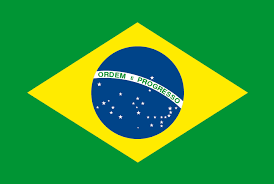
\includegraphics[width=8cm]{pictures/flaga.png}
    \caption{Flaga Brazylii}
    \label{fig:flaga}
\end{figure}

\section{Lista numerowana}
Lista krajów Ameryki Południowej
\begin{enumerate}
    \item Brazylia (Patrz Rysunek \ref{fig:flaga})
    \item Argentyna
    \item Chile
    \item Urugwaj
    \item Paragwaj
    \item Boliwia
    \item Peru
    \item Kolumbia
    \item Wenezuela
    \item Ekwador
    \item Gujana
    \item Surinam
\end{enumerate}

\section{Lista nienumerowana}
Przykładowe sporty
\begin{itemize}
    \item Piłka nożna
    \item Siatkówka
    \item Koszykówka
    \item Golf
    \item Bieganie
\end{itemize}